\documentclass[runningheads]{llncs}
\usepackage{bm}
\usepackage{CJK}
\usepackage{graphicx}
\usepackage{subfigure}
\usepackage{tikz}
\usetikzlibrary{fit,positioning}

\begin{document}
\title{Explain urban regional function}
\author{Submission}

\maketitle

\begin{abstract}
Functional region identification is a critical step towards Urban computing.
The state-of-the-art Dirichlet Multinomial Regression(DMR) has identify regions with different function based on topic cluster modeling.
Due to the ingenious structure inside the complex model, its result is beyond the direct comprehension of humans.
How to give them reliable explanations are the main objectives of this work.
To improve the persuasiveness of its result, we proposed a post hoc framework to make explanation for it.
Optimal latent factor model was applied as explanation after the identification.
We use matrix factorization to get latent factors and correlate latent factors with urban feature.
The selected urban feature can be labeled as the explanation.
Our framework can give an strong evidence to the identification and enhance the satisfaction of users and system designers.

(15--250 words.)

\keywords{Explainable AI  \and Urban computing \and Online Sentiment analysis \and Big data analysis \and Functional region identification}
\end{abstract}
%


\section{Introduction}
%urban computing
Urban computing is a process to acquire, integrate and analyze big and heterogeneous data generated by diverse sources in urban spaces~\cite{Zheng2014UrbanConcepts}. 
Recently, urban computing has attracted attentions from both academy and industry.
One critical step towards efficient urban computing is to identify \emph{functional regions}, which are regions in a city that support certain needs of urban lives~\cite{Yuan2012FunctionRegion,Yuan2015FunctionRegion}.

%related work survey
Most of previous \emph{Functional Region Identification} (FRI) systems use clustering methods on mobility data~\cite{Karlsson2006FunctionalRegionSummary}.
For example, clustering algorithm based on the 'modularity function' is applied on telecommunication data~\cite{Newman2004ModularityFunction,Ratti2010Telecom}, spectral clustering is applied on remote-sensor image data~\cite{Vatsavai2011Remote}, variants of Latent Dirichlet Allocation (LDA) is applied on remote-sensor data~\cite{Vatsavai2010Remote} and taxicab pick-ups and drop-offs data~\cite{Yuan2012FunctionRegion,Yuan2015FunctionRegion}.

%problem of past research
A severe drawback of existing research is the lack of explanation for functional regions.
Clustering methods generate cluster labels that have long been suffering from the subjective issue, i.e. the system only provides one possible partitioning of the regions while the users have no idea what the partitioning means. 
Furthermore, to obtain accurate identification, recent research tends to use complex models such as the Dirichlet Multinomial Regression model in~\cite{Yuan2015FunctionRegion} . 
The complex nature of these models is an obstacle for people to capture the ``semantics'' of the clustering results. 

%motivation
There is a strong incentive to develop explainable FRI system, which \emph{explains} the identification of functional regions. 
Explainable FRI is beneficial for both system designers and end users.
For system designers, providing explanations help them better diagnose the system and improve system performance. 
For end users, explanations not only facilitate interpretation of the clustering results, but also incubate a wide range of applications, including traffic flow predictions, personalized trajectory recommendation, urban planning and so on. 

%goal
Though there is a growing interest in studying explainable AI~\cite{Preece2018ExplainAI}, in geographical systems, explainable system is still in its initial stage~\cite{Korpan2017navigation,Jose2018cognitive}.
In this paper, we present a novel system for explainable FRI by integrating heterogeneous data sources. Our system provides post-hoc explanations, i.e. the explanations are not relevant to the FRI algorithm. Instead, for an arbitrary FRI algorithm, the system attempts to resolve the ``semantics" of the generated cluster labels by (1) associating the cluster labels to a set of human activities; (2) visualizing the desired urban features for each activity; and (3) listing the most important urban features in the region. 

%figure ??? real example or made-up example
As shown in Fig.\ref{explanation-example}, the city has been partitioned into several functional regions. For a specific region $r_1$ with label $I$, the system delivers textual and visual descriptions. Firstly label $l$ is most likely to relate to a mixture of activities ``'' and ``'', because from the analysis of mobility data, these two activities bring in $\%$ of the traffic flow to region $r_1$. Secondly, under activity ``", two urban features ``'' and ``" are most popular, with highly positive sentiments collected from online reviews. Finally region $r_1$'s most representative urban features are exactly ``" and ``", thus the system \textbf{explains} why $r_1$ is labeled as $l$.  

%highlight
We highlight a key property of the proposed system: the power to integrate heterogenous data sources. On one hand, explanations essentially involve semantics. In our system, the semantics of labels are expressed through urban activities and urban features, which are extracted from online review data. On the other hand, the cluster labels are obtained in mobility data. To obtain more reasonable explanations that comply with the clustering algorithm, the semantics are blended with moving patterns discovered in mobility data. In building such a system, we face two challenges.

\begin{figure}
\centering
\subfigure[An example of our identification result]{
\label{real-map} %% label for first subfigure
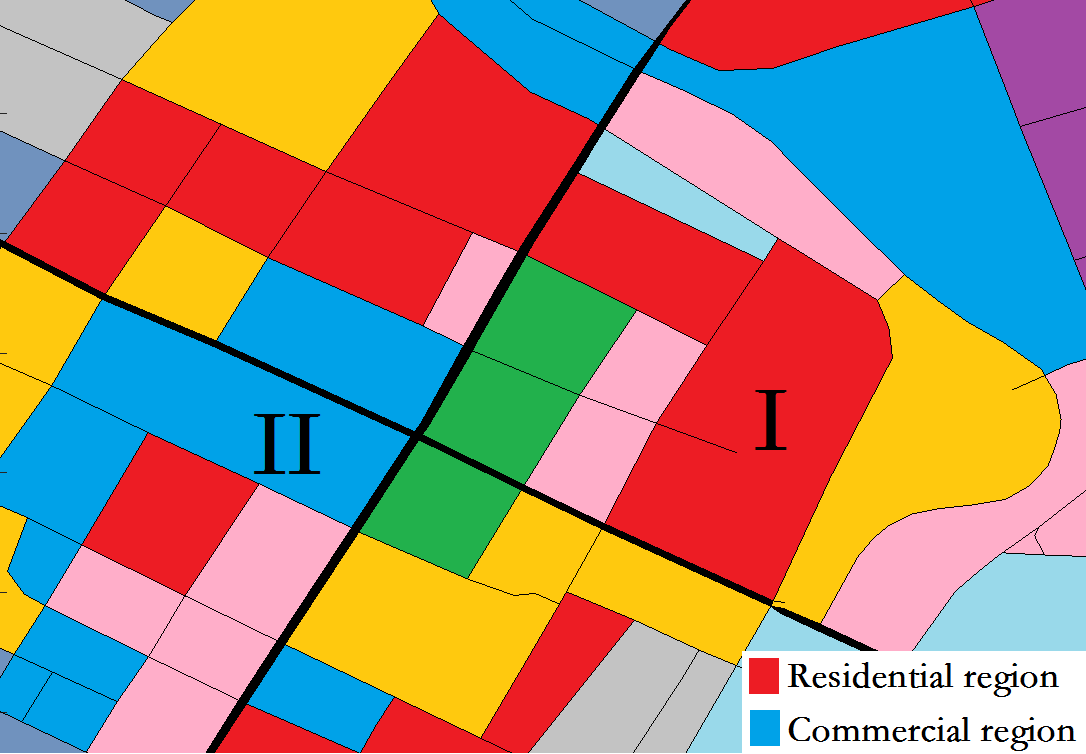
\includegraphics[width=1.5in]{example-net.png}}
\subfigure[moving patterns]{
\label{patterns} %% label for second subfigure
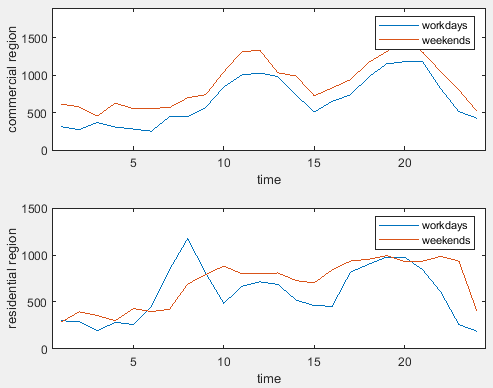
\includegraphics[width=1.4in]{example-line.png}}
\subfigure[POIs in different functional region]{
\label{sentiment} %% label for second subfigure
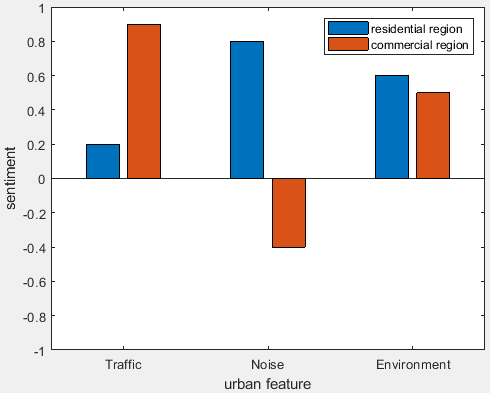
\includegraphics[width=1.4in]{example-sentiment.png}}
\caption{The explanation provided for functional region identification.
Region I in Fig.\ref{real-map} is labeled as residential region while II is commercial region.
Fig.\ref{patterns} revealed differences of the mobility patterns between residential region and commercial region,workdays and weekends.
Fig.\ref{POI} shows the distribution of POIs within the two regions,e.g. there is more shops in commercial region.
And from fig.\ref{sentiment} we find that people have a more interest in a positive sentiment in traffic for commercial and pay more attention to noise for residential region.}
\label{explanation-example} %% label for entire figure
\end{figure}

%manual label costly supervision in sufficient
The first one of it is to extract the urban feature from comment data.
Urban feature is a set of characters with special geographical attributes, e.g., clothes, school, bars and so on.
Most of our content data are comments of shops with the shop address.The feature extracted from it is more related to shop feature than urban feature.
Therefore, existing sentiment extraction model ~\cite{Lu2011Label} can not be used directly in our models.%urban feature
In order to get the location information from these content data, all features are extracted as~\cite{Zhang2015Sentires}.
We select typical features with a high frequency and high information entropy from it.

%unsupervised

%how to embed mobility data
And the second challenge is how to explain the features.
If the extracted urban features used for explanations can not correspond to the labeled activity used to identify functional regions, the explanations will not have a strong explanation power for the identification, or even will not be generated.
To improve the explanation power of our framework, we extract related urban feature and find the corresponding sentiment score between activity and urban feature from contents.
With the probability that region units belong to which function generated by DMR, we can applied matrix factorization to find the relativity between region units and latent factor, i,e urban feature.
The urban feature with highest relativity make an explanation for why corresponding region units are identified as such function.

%bias curve

\textbf{Contribution.}
Our paper has an outstanding result in following several aspect:
\begin{itemize}
  \item To the best of our knowledge,we are the first to give explanation to urban functional region identification , which could improve the trustiness and satisfaction of users and urban system designers.
  \item After identify different functions, We use the contents with sentiment to find the typical urban feature within a region and make explanation.
  \item The explanation is given by latent factor model. We appplied matrix factorization to get the correlation coefficients between single region units and its features.
\end{itemize}


The remainder of the paper is organized as follows.
We give an overview for related work in Section 2.
In Section 3, we give an overview of our framework.
Section 4 shows the process of functional region identification as well as urban feature extraction.
And Section 5 introduces the post hoc explanation model.
We test the framework on our datasets and presents the superior explanation result in Section 6
Finally, we made a conclusion and looked forward to our future work in Section 7.

\section{Related Work}
Our work is build upon taxicabs trajectory and comment text.
With the data source, two lines of work are related to this paper: urban computing and online sentiment analysis .

%related work section name, find another suitable name for mobility mining
\subsection{Urban Computing}

Urban computing~\cite{Zheng2014UrbanConcepts} tackles the major issues that cities face by analyzing human mobility collected from different sensors.
Major sources of human mobility data are check-ins in POI~\cite{Gallegos16happier}, pick-up and drop-off behavior of taxicabs~\cite{Ge2011TaxiBusiness,Meng2017Traffic} in different locations and  trajectories.

%extract the different among these data
The simplest form of mobility data is \textbf{check-ins data}, which are collected from locating sharing services. Check-ins data usually includes a set of point revealing users' current location.
Statistical association analysis is commonly conducted on check-ins. For example, radius of gyration is measured in~\cite{Cheng2011Check-in}, which is extended by combining with lexicon into demographics~\cite{Gallegos16happier}.
A few recent work adopts model based approaches, e.g. context-aware tensor factorization that take account of contextual factors that influence consumers refueling decision~\cite{Zhang2015Fuel}.

The second form of mobility data is \textbf{origin-destination pairs}, i.e. a pick-up point and a drop-off point of a taxi trajectory.
Clustering methods including Newman modularity cluster algorithm~\cite{Newman2004ModularityFunction} are applied in functional region identification~\cite{Ratti2010Telecom}.
Recently, latent factor models are proposed to treat a region as document and infer functional-specific ~\cite{Yuan2012FunctionRegion}.%
Latent activity is imported in topic model in~\cite{Yuan2015FunctionRegion} to define the specific functions of different regions.

Alternatives for origin-destination pairs are \textbf{trajectory data}.
Applications on trajectory data include recommendation, e.g. to recommend more suitable place to drivers~\cite{Ge2011TaxiBusiness,Garg2018Route} and traffic planning, e.g. to find reachable region within a given temporal period~\cite{Wu2017Reachable}, %find a fast route
or to predict travel time~\cite{Wang2018Deep}.

In early work, a functional region was defined as a geographical region where the majority of local population recruit and are employed within the region \cite{Ball1980Definition}.
Due to the availability of large-scale mobility data, an increasing amount of data-driven approaches~\cite{Farmer2009Overview} have been proposed.
Most of them use clustering methods on commuting data, such as origin-destination pairs of labour market data ~\cite{Karlsson2006FunctionalRegionSummary} while others use remote-sensor image data~\cite{Vatsavai2011Remote}.
Later work focuses on city-level functional region identification,

%tasks
However, existing urban computing systems extensively rely on complex machine learning algorithms hence they act as blank-boxes for end users.
The lack of explanation weakens the persuasiveness and trustworthiness of the system for users.
Our work is to make up for this drawback by providing intuitive explanations of the results for users or system designers

\subsection{Geographical Analysis of Online Sentiment}

Recently, an emerging research interest is witnessed in exploring the geographical factors that affect online sentiment.
Empirical studies have been conducted on large-scale human mobility data, such as check-in ~\cite{Gallegos16happier}and trajectory~\cite{Gonzlez2008Track},to find the geographical content analysis with sentiment.
Associations are found between online sentiments and geographical factors, e.g happy regions are more likely to connect with each other~\cite{Alshamsi15milan},a high check-in density region usually presents a more positive mode~\cite{Gallegos16happier}, the whole process and development of a organized movement could be tracked on the social media~\cite{Alvarez2015Movement} and so on.

%and emotion
%complete survey
However, most existing work of this line employ simple statistical analysis to uncover the associations.
Such a coarse-grained analysis is distorted by latent variables, such as activity of the region.
Our work is the first to incorporate activity to obtain a fine-grained analysis.






















\section{System Overview}
The section make an overview introduction for our post hoc framework to explain the functional region identification.
The whole structure is illustrated in Figure ~\ref{overview} while the corresponding steps as follow:

\begin{figure}[h]
  \centering
  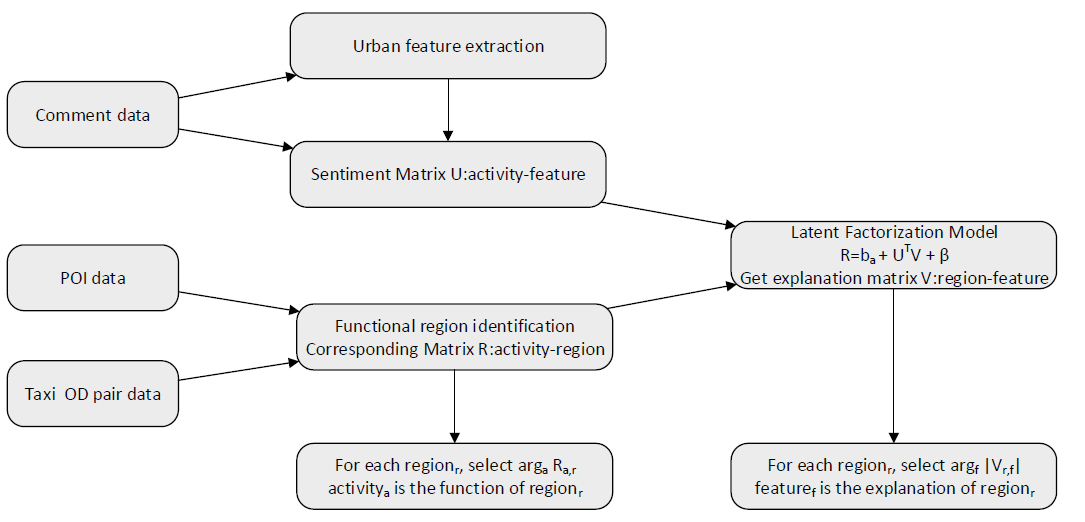
\includegraphics[scale=0.3]{overview.png}
  \label{overview}
  \caption{The overview structure of our framework}
\end{figure}

\emph{1.Functional region identification:}

The input data of first step is taxicabs OD pairs and POIs with coordinates.
We can get an activity-region matrix with value of the probability that each single region units belong to each activity by DMR.
And for the region, an activity with highest probability can be output as the function of this region.

\emph{2.Urban feature extraction:}

This step based upon the comments of different shops and activity-region matrix output in last step.
We select nouns with high frequency and low information entropy as our urban features.
Meanwhile, the sentiment analyse between urban feature and different activity is also illustrated in an activity-feature matrix.

\emph{3.Train Matrix Factorization model:}

With the certain activity-region matrix $\bm{r}$ and activity-feature matrix $\bm{u}$, we performed an matrix factorization model in form of Equation \ref{model} to get the region-feature matrix $\bm{v}$.
Training data comes from the given result of step 1 and step 2.

\emph{4.Output label explanation:}

The region-feature matrix $\bm{v}$ generated in step 3 in the input of this step
For each single region units,we can pick the urban features with highest sentiment score in $\bm{v}$.
These urban feature is the explanation for the functional region identification.




















\section{Urban Feature}
\subsection{Functional Region Identification}
A city was segmented into single region units, which is regarded as documents with various themes in topic modeling.
DMR~\cite{Mimno2012DMR} was applied in functional region identification as explained in~\cite{Yuan2012FunctionRegion}.
DMR, whose structure is illustrated in Figure~\ref{DMR_ori}, is a topic clustering model based on Latent Dirichlet Allocation(LDA).
It input some metadata, e.g. authors and publishers, in addtion to basic LDA, which make the topic modeling more accurate.
As describe in~\cite{Yuan2012FunctionRegion},we regard flow increment calculated in regions as vocabulary in documents, which is marked as $m_{r,n}$ in Figure~\ref{DMR_ori}.
And POI located in different region units are correlate to the matadata of document, which is marked as $x_r$ in Figure~\ref{DMR_ori}.
\begin{figure}[h]
  \centering
  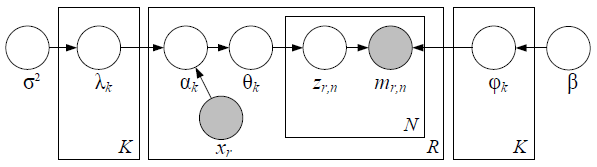
\includegraphics[scale=0.4]{DMR.png}
  \caption{The structure of DMR}
  \label{DMR_ori}
\end{figure}

\subsection{Urban Feature Extraction}
To get proper urban features for explaining different functions, we thought that urban features should be nouns with high frequency and low information entropy.

Considering the property of urban features, we separate comment sentences into single words and select all nouns of it.
With the help of coordinates, these words can correspond to different single units.
Take the sparseness of latent factor into account, we thought the words had better appear in more region units.
And we filer the high-frequency nouns as features.
If the frequency of a word is high enough, i.e. the shops commented with this word is much than a threshold $t$, we thought its frequency is high.
We set the threshold $t$ as 500.

Meanwhile, to make the urban features more distinguishing, we calculate the information entropy of words for different functional regions generated in Section 4.1.
Information entropy can measure the amount of information that a word contains.
Stronger distinguishing ability of a word takes lower information entropy.
The information entropy is defined as:
$$H[x_i,word_j] = -\sum_i p(x_i,word_j)\log p(x_i,word_j)$$
where $x_i$ stands for $i$th functional regions;
$p(x_i,word_j)$ is the proportion of shops located in $i$th functional regions commented with $j$th word in all shops located in $i$th functional regions.
We select features with lowest information entropy as our urban features, which are shown in Table \ref{urbanfeatures}.

\begin{table}[h]
\centering
\caption{Selected Urban Features}
\label{urbanfeatures}
\begin{tabular}{c|c|c|c|c}
\hline
features &  Alley & Brand & Center & Square\\
\hline
information entropy &  &  &  & \\
\hline
\end{tabular}
\end{table}


\subsection{Urban Feature Matrix}

















\section{Explanation Model}
In this section,we describe our post hoc framework for explanation in detail.

\subsection{Latent Factor Model}
A classical model has Intuitive explanation is latent factor model.
It has a wide application in various fields.
The form of latent factor applied in recommendation system to predict rating of user $u$ to product $p$ as follow:
\begin{equation}
\hat{r}_{u,p}= g+b_u+b_p+\bm{x_u}^T\bm{y_p} \label{basic}
\end{equation}
where $g$ is a base rating in the system while $b_u$ and $b_p$ is the bias of user $u$ and product $p$;
$\bm{x_u}$ and $\bm{y_p}$ denote vectors of latent factors for corresponding user and product.

The matrix $r$ is rating that user $u$ give to product $p$.
Correlate users as activities, products as locations, we translated the matrix into the sentiment analysis score that actitivy $a$ to region $l$.
We can make our matrix based upon this stand latent factor model presented in Equation \ref{basic}.

\subsection{Our model}
Considering the temporal attribute of datesets, ~\cite{Zhang2017Model} has proposed an Historical Influence Aware Latent Factor(HIALF) model take the historical influence into account, which fit our intuition well and make the power of explanation stronger.

Therefore, we define our matrix factorization model as:
\begin{equation}
\hat{r}_{l,i,a}=b_l+U_a^TV_l+\beta(e_{a,i})\label{model}
\end{equation}
where $\hat{r}_{l,i,a}$ stands for the predicted probability at $i$-th time bin that region $l$ belongs to activity $a$;
$b_l$ is the bias of region $l$;
$\bm{U_a}$ and $\bm{V_l}$ represent the latent feature of activity $a$ and region $l$;
$e_{a,i}$ generated by prior expectation;
and $\beta(\cdot)$ demonstrates the bias curve changing with $e_{a,i}$.
Now we describe how to learn the $\beta(x)$ and generate a more realistic prior expectaion $e_{a,i}$.

\textbf{Modeling the bias curve $\beta(x)$}
The form of $\beta(x)$ is unknown.
We can constrain it with a data-driven approach.
Kernel regression is a kind of typical non-parameter learning and fit the $\beta(x)$ model well.

If we have a set of independent variables $e_l$ and dependent variables $v_l$, and $v_l=\beta(e_l)+\epsilon_l$ where $\epsilon_l$ is the noise from the standard normal distribution, we can defind $\beta(x)$ as:
$$\beta(x) = \frac{\sum_{k=1}^{n}w(x,e_l)v_l}{\sum_{k=1}^{n}w(x,e_l)}$$
where $w(x, x_i) = \exp(-\kappa(x-x_i)^2)$ and $\kappa$ is given by 10.
Actually, $e_l$ is given while $v_l$ is unknown.
Therefore, we set $e_l$ as several arithmetic progression within data range and $v_l$ is the corresponding unknown parameters so that we can learn them from datasets.

\textbf{Modeling the prior expectation $e_{a,i}$}
$$e_{a,i} = \frac{\sum_{k=1}^{i-1}\xi(i-k) r_{a,k}}{\sum_{k=1}^{i-1}\xi(i-k)}$$
where $\xi(d)=\exp(-\gamma\times d)$ is an exponential triggering kernel that models the decrease of histroy influence;
$\gamma$ controls the degree that history probability influence current probability;
and $r_{a,k}$ denotes the sentiment of activity $a$ when time bin $k$.


\subsection{Model Inference}
After build a matrix factorization model, we set up objective function as follow:
\begin{equation}
F=\sum\limits_{(p,l,u)\in\mathcal{M}}(r_{l,i,a}-\hat{r}_{l,i,a})^2+\lambda_1(b_l^2+||{\bm{y_r}}||_2^2)+\lambda_2(\sum\limits_{l}v_l^2)+\lambda_3(\sum\limits_{\alpha}\alpha_u^2)
\label{inference}
\end{equation}
where $\Theta$ stands for the unknown parameters, $\bm{y_p}$, $b_u$, $\alpha$ and $v_l$.
$\mathcal{M}$ contains all $(p,l,u)$ pairs, and each pair of it stands for the related parameter of region $l$ belongs to activity $a$ at time bin $i$.
$r_{r,i,a}$ is the probability generated by DMR while $\hat{r}_{r,i,a}$ is the predicted probability by Equation \ref{model}.
The first item of Equation \ref{inference} is quadratic sums of the difference between real probability $r_{r,i,a}$ and predected probability $\hat{r}_{r,i,a}$.
To prevent from overfitting, we three regularization terms and $\lambda_1$, $\lambda_2$ and $\lambda_3$ are given as hyperparameters.


To get our optimal $\bm{y_r}$, we aim to solve the following optimization problem and make the predicted probability $\hat{r}_{r,i,a}$ as close as possible to the real probability$r_{r,i,a}$:
$$\min\limits_{\Theta} F$$
The approach to get it is stochastic gradient descent(SGD) algorithm due to its efficiency in learning the parameter of objective function























\section{Experiments}
\subsection{Data Set}
The data set for our experiments including both mobility data and content data.
The mobility data including the pick-up and drop-off timestamps and coordinates in November of the year 2016 provided by DiDi, the biggest taxi platform in China.It contributed to the movement pattern of human mobility.
And the online content is crawled from a website with many comments similar to Yelp called DazhongDianping, which helps sentiment analysis of the regions.
\begin{table}[h]
\caption{Statistics of datasets}\label{dataset}
\begin{tabular}{|l|l|c|}
\hline
Datasets &  attributes & Value\\
\hline
comments & shops with coordinates(POI) & 109686\\
 & shops with comments & 50853\\
 & total comments & 3213264\\
\hline
taxicabs & effective orders & 7065937\\
 & effective days & 30 \\
\hline
road networks & geographical scope & [103.93$^\circ$E,104.21$^\circ$E] and [30.56$^\circ$N,30.79$^\circ$N]\\
 & road segments & 3712\\
 & percentage of major roads & 54.9\%\\
 & segmented regions & 901\\
\hline
\end{tabular}
\end{table}

\subsection{Preparation}
To form the basic region of city,we segment the urban area of city into region units by the major road network and make a map simplification.
The longitude of map range is [103.93,104.21] and latitude range is [30.56,30.79], which covers the main area of a city.
Raster-based model is more computationally efficient and succinct for territorial analysis, which is suitable for our map scenario.
We downloaded the major road network of this region\footnote{http://www.bigemap.com/} and rasterized the area into a 2000 $\times$ 2400 grid.
In the grid, the road network is converted to a binary image, as 1 stands for the road while 0 stands for the blank areas.

The main road data is present in Fig.\ref{raw_map}, including motorway, trunk, primary, secondary, tertiary and their links.
But the Fig.\ref{raw_map} is full of some unnecessary details, such as the lanes of a road and the overpasses, which disturb the distribution of regions.
As explained in~\cite{Yuan2015FunctionRegion}, the dilation and thinning process illustrated in Figure~\ref{dilation and thinning} are operated on the original road data to remove some small regions and simplify the map.
\begin{figure}[h]
    \centering
    \subfigure[Original segment of city]{
    \label{raw_map} %% label for first subfigure
    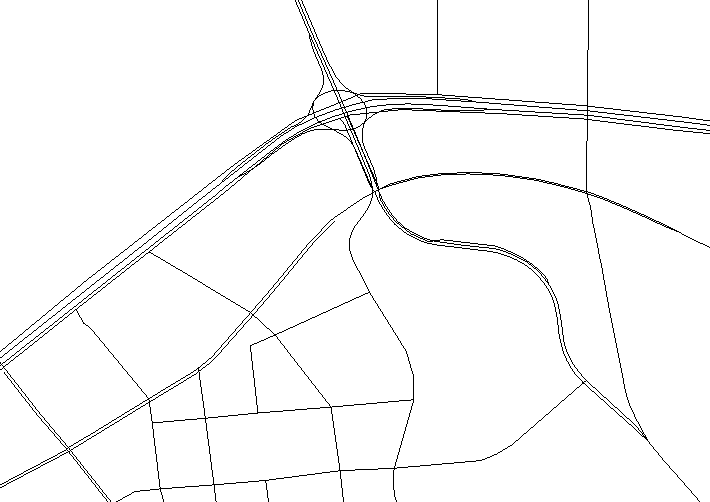
\includegraphics[width=1.5in]{chengdu_1.png}}
    \subfigure[After dilation operator]{
    \label{dilation} %% label for second subfigure
    
\includegraphics[width=1.5in]{chengdu_2.png}}
    \subfigure[After thinning operator]{
    \label{thinning} %% label for second subfigure
    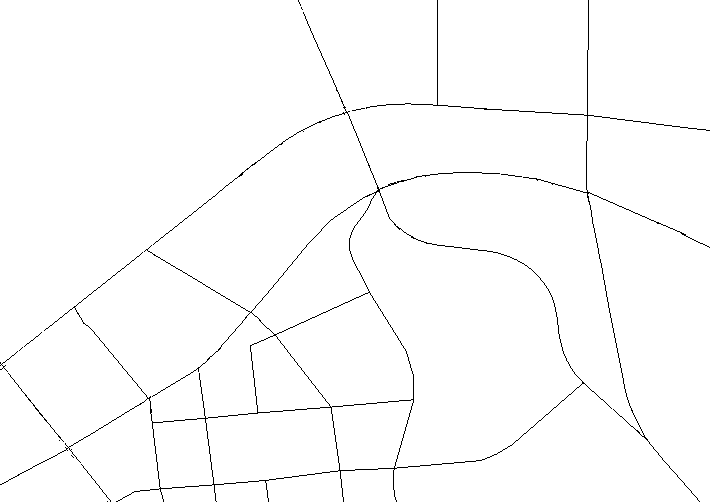
\includegraphics[width=1.5in]{chengdu_3.png}}
    \caption{The preparation process of road network}
    \label{dilation and thinning} %% label for entire figure
\end{figure}

We use DMR to identify regions into 8/4 types with different regions, which is illustrated in Figure~\ref{DMR_result}
The main function regions in the city is residence region, business region, study and science region, scenery regions and so on.

\begin{figure}[h]
\centering
\subfigure[After dilation operator]{
\label{thin_result} %% label for second subfigure
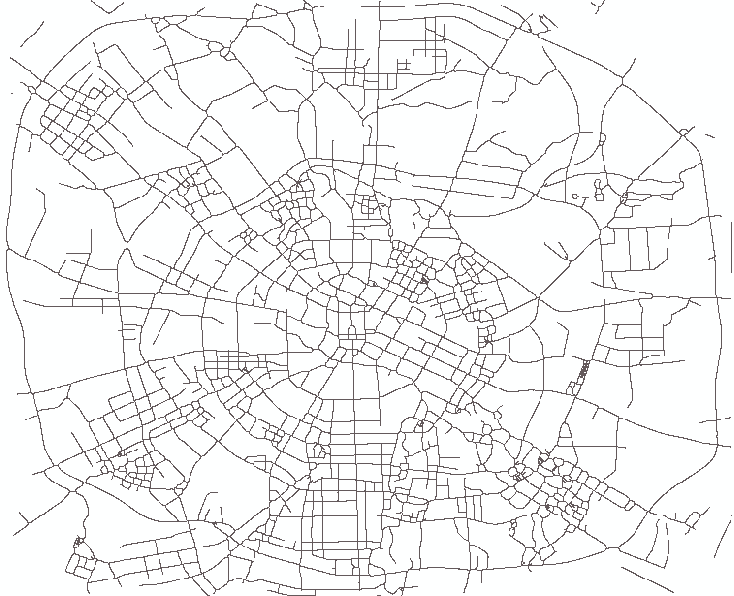
\includegraphics[width=2.3in]{FunctionalRegions_thinning.png}}
\subfigure[segmented region units of the city]{
\label{DMR_result} %% label for second subfigure
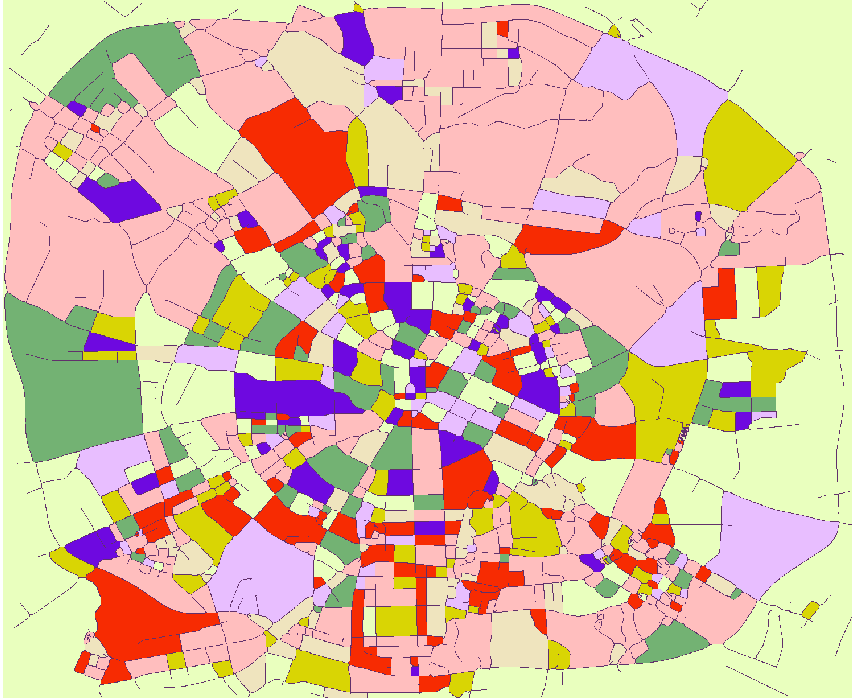
\includegraphics[width=2.3in]{FunctionalRegions_DMR.png}}
\caption{results of DMR}
\label{The results of functional region identification}
\end{figure}

\subsection{Evaluation Metrics}
We evaluate the functional region through two approaches. One is the percentage of regions that could find explanation label by our framework; while the other is the quality and accuracy of the explanation given by our framework.

For the evaluation of percentage of explainable region, we put forward the $explanation percentage$ to measure the proportion that regions with explainable labels as:
$$explanation\ percentage=\frac{|regions\ with\ explanation\ label|}{|all\ regions|}$$

For the second approach,we take a metric to measure the quality and accuracy of our explanation label.

\subsection{Baseline and other comparison}

\subsection{result}
\begin{table}[h]
\centering
\caption{Functional Regions and corresponding urban feature}\label{dataset}
\begin{tabular}{c|c}
\hline
Functions & Urban Feature\\
\hline
Business & \\
\hline
Residence & \\
\hline
Study & \\
\hline
Scenery & \\
\hline
\end{tabular}
\end{table}

\section{Conclusion}
Function regions identification is an important part of urban computing.
But its evaluation depend on human intuition and urban planning, which is hard to display in terms of statistics.
To make up for the lack of persuasive explanation, we proposed a post hoc framework to give persuasive explanation for functional regions identification in this paper.
Our datasets including over 3 million comments of shops and taxicabs OD pair trajectory in November 2016 generated by more than 7 million orders.
We utilized the framework to general most relative labels for every single region units as explanation.
According to the experiments performed in the datasets, our framework give an strong evidence to the identification and enhance its persuasiveness.
The result can help users and urban system designers easily recognize the region functions, which is helpful in a variety of urban applications, such as urban planning, location choosing for a business advertisement casting, and so on.

There are some directions can improve in the future work.
First is to full utilize our data sets of trajectory. 
Our trajectory datasets not only have origin and destination, but also include the detail points that users have passed by.
There are also some interesting patterns within these process points, and we can find new moving patterns in it. 
Second, we want to change our phrase-level explanation into sentence-level, which is more similar to natural language.



\begin{thebibliography}{25}
\bibitem{Zheng2014UrbanConcepts}Zheng Y, Capra L, Wolfson O, et al. Urban Computing:Concepts, Methodologies, and Applications[J]. Acm Transactions on Intelligent Systems \& Technology, 2014, 5(3):1-55.
  
\bibitem{Zheng2011taxicabs}Zheng Y, Liu Y, Yuan J, et al. Urban computing with taxicabs[C]// International Conference on Ubiquitous Computing. ACM, 2011:89-98.
   
\bibitem{Meng2017Traffic}Meng, C.; Yi, X.; Su, L.; Gao, J.; Zheng, Y. City-wide Traffic Volume Inference with Loop Detector Data and Taxi Trajectories. Proceedings of the 25th ACM SIGSPATIAL International Conference on Advances in Geographic Information Systems,ACM,2017, 1:1-1:10


\bibitem{Vatsavai2011Remote}Vatsavai R R, Bright E, Varun C, et al. Machine learning approaches for high-resolution urban land cover classification:a comparative study[C]// International Conference and Exhibition on Computing for Geospatial Research \& Application, Com.geo 2011, Washington, Dc, Usa, May. DBLP, 2011:1-10.

\bibitem{Vatsavai2010Remote}Vatsavai R R, Cheriyadat A, Gleason S. Unsupervised Semantic Labeling Framework for Identification of Complex Facilities in High-Resolution Remote Sensing Images[C]// IEEE International Conference on Data Mining Workshops. IEEE Computer Society, 2010:273-280.
 

\bibitem{Ratti2010Telecom}Ratti C, Sobolevsky S, Calabrese F, et al. Redrawing the Map of Great Britain from a Network of Human Interactions[J]. Plos One, 2010, 5(12):e14248.

\bibitem{Yuan2010NextPassenger}Yuan J, Zheng Y, Zhang L, et al. Where to find my next passenger[C]// Proceedings of the 13th international conference on Ubiquitous computing. ACM, 2011:109-118.
\bibitem{Ge2011TaxiBusiness}Ge Y, Liu C, Xiong H, et al. A taxi business intelligence system[C]// ACM SIGKDD International Conference on Knowledge Discovery and Data Mining, San Diego, Ca, Usa, August. DBLP, 2011:735-738.
\bibitem{Farmer2009Overview}Farmer, C. J. (2009). Data driven functional regions. In Proceedings of 10th International Conference on GeoComp
 
\bibitem{Garg2018Route}Nandani Garg and Sayan Ranu. Route Recommendations for Idle Taxi Drivers: Find Me the Shortest Route to a Customer!. In KDD 18: The 24th ACM SIGKDD International Conference on Knowledge Discovery \& Data Mining, August 19-23, 2018, London, United Kingdom. 2018.

\bibitem{Goddard1970EarliestFunction}Goddard J B. Functional Regions within the City Centre: A Study by Factor Analysis of Taxi Flows in Central London[J]. Transactions of the Institute of British Geographers, 1970, 49(49):161-182.
 
\bibitem{Karlsson2006FunctionalRegionSummary}Karlsson C, Olsson M. The identification of functional regions: theory, methods, and applications[J]. Annals of Regional Science, 2006, 40(1):1-18.
   
\bibitem{Newman2004ModularityFunction}Newman M E J. Detecting community structure in networks[J]. European Physical Journal B, 2004, 38(2):321-330.
   
\bibitem{Ball1980Definition}R.M. Ball. The use and definition of Travel-to-Work Areas in Great Britain: Some problems[J]. Regional Studies, 1980, 14(2):125-139.
\bibitem{Yuan2012FunctionRegion}Yuan J, Zheng Y, Xie X. Discovering regions of different functions in a city using human mobility and POIs[C]// ACM SIGKDD International Conference on Knowledge Discovery and Data Mining. ACM, 2012:186-194.

\bibitem{Yuan2015FunctionRegion}Yuan N J, Zheng Y, Xie X, et al. Discovering Urban Functional Zones Using Latent Activity Trajectories[J]. Knowledge \& Data Engineering IEEE Transactions on, 2015, 27(3):712-725.
  
\bibitem{Yuan2018FunctionRegion}Yuan N J, Zheng Y, Xie X. Discovering Functional Zones in a City Using Human Movements and Points of Interest[J]. 2018.

\bibitem{Zhang2015Fuel}Zhang F, Yuan N J, Wilkie D, et al. Sensing the Pulse of Urban Refueling Behavior:A Perspective from Taxi Mobility[J]. Acm Transactions on Intelligent Systems \& Technology, 2015, 6(3):1-23.
 
\bibitem{Shang2014Pollution}Shang J, Zheng Y, Tong W, et al. Inferring gas consumption and pollution emission of vehicles throughout a city[J]. 2014:1027-1036.

\bibitem{Wu2017Reachable}Wu G, Ding Y, Li Y, et al. Mining Spatio-Temporal Reachable Regions over Massive Trajectory Data[C]// IEEE, International Conference on Data Engineering. IEEE, 2017:1283-1294.
 
\bibitem{Wang2018Deep}D Wang,J Zhang,W Cao,J Li,Y Zheng.When Will You Arrive? Estimating Travel Time Based on Deep Neural Networks.In International AAAI Conference on Web and Social Media, 2011.
 
\bibitem{Alvarez2015Movement}R. Alvarez, D. Garcia, Y. Moreno, and F. Schweitzer. Sentiment cascades in the 15m movement. EPJ Data Science, 4(1):1-13, 2015

\bibitem{Alshamsi15milan}Alshamsi A, Awad E, Almehrezi M, et al. Misery loves company: happiness and communication in the city[J]. Epj Data Science, 2015, 4(1):7.

\bibitem{Cheng2011Check-in}Z. Cheng, J. Caverlee, K. Lee, and D. Sui. Exploring millions of footprints in location sharing services. In International AAAI Conference on Web and Social Media, 2011.

\bibitem{Gonzlez2008Track}Gonzlez M C, Hidalgo C A. Understanding individual human mobility patterns[J]. Nature, 2008, 453(7196):779-782.

\bibitem{Gallegos16happier}Gallegos L, Huang A, Huang A, et al. Geography of Emotion: Where in a City are People Happier?[C]// International Conference Companion on World Wide Web. International World Wide Web Conferences Steering Committee, 2016:569-574.

\bibitem{Zhao2016POI}Zhao S, King I, Lyu M R. A Survey of Point-of-interest Recommendation in Location-based Social Networks[J]. 2016.

\bibitem{Zhang2018SIGIR}Yongfeng Zhang, Yi Zhang, and Min Zhang. SIGIR 2018 Workshop on ExplainAble Recommendation and Search (EARS 2018). In Proceedings of The 41st International ACM SIGIR Conference on Research and Development in Information Retrieval (SIGIR 18). 2018.

\bibitem{Zhang2018Survey} Zhang Y, Chen X. Explainable Recommendation: A Survey and New Perspectives[J]. arXiv preprint arXiv:1804.11192. 2018.
  
\bibitem{Herlocker2000Explanation} Herlocker J L, Konstan J A, Riedl J. Explaining collaborative filtering recommendations[C]// Acm Conference on Computer Supported Cooperative Work. 2000:241-250.
 
\bibitem{Ferwerda2012ContentCorrelate} Ferwerda B, Swelsen K, Yang E. Explaining Content-Based Recommendations[J]. Bruceferwerda Com.
 
\bibitem{Zhang2015Sentires}  Zhang Y, Zhang M, Liu Y, et al. Boost Phrase-level Polarity Labelling with Review-level Sentiment Classification[J]. Computer Science, 2015.
    Zhang Y, Lai G, Zhang M, et al. Explicit factor models for explainable recommendation based on phrase-level sentiment analysis[C]// International Acm Sigir Conference on Research \& Development in Information Retrieval. ACM, 2014:83-92.

\bibitem{Costa2017LSTM} Costa F, Ouyang S, Dolog P, et al. Automatic Generation of Natural Language Explanations[J]. 2017
\bibitem{Preece2018ExplainAI}Preece A. Asking 'Why' inAI: Explainability of intelligent systems - perspectivesand challenges. Intell Sys Acc Fin Mgmt. 2018;25:63-72.
    %explain AI
\bibitem{Korpan2017navigation}Korpan, R., Epstein, S.L., Aroor, A., Dekel, G.: WHY: Natural explanations from a robot navigator. In: AAAI 2017 Fall Symposium on Natural Communication for Human-Robot Collaboration.
\bibitem{Jose2018cognitive}Jose M. Alonso, Corrado Mencar. Building Cognitive Cities with Explainable Artificial Intelligent Systems. In Proceedings of the First International Workshop on Comprehensibility and Explanation in AI \& ML, 2017.
\bibitem{Lu2011Label}Lu Y, Castellanos M, Dayal U, et al. Automatic construction of a context-aware sentiment lexicon:an optimization approach[C]// International Conference on World Wide Web, WWW 2011, Hyderabad, India, March 28 - April. DBLP, 2011:347-356.
\bibitem{Zhang2017Model}Zhang X , Zhao J , Lui J C S . Modeling the Assimilation-Contrast Effects in Online Product Rating Systems: Debiasing and Recommendations[C]// Eleventh Acm Conference on Recommender Systems. ACM, 2017.
\bibitem{Mimno2012DMR}Mimno D, Mccallum A. Topic Models Conditioned on Arbitrary Features with Dirichlet-multinomial Regression[J]. University of Massachusetts - Amherst, 2012, 2008:411--418.
\end{thebibliography}
\end{document}
